\documentclass[tikz,border=6pt]{standalone}
\usepackage{pgfplots}
\pgfplotsset{compat=1.18}
\usepgfplotslibrary{colormaps}
\usetikzlibrary{arrows, arrows.meta, calc}
\usetikzlibrary{decorations.markings}


\usepackage{amssymb,amsmath,mathtools}

\usepackage[T1]{fontenc}
\usepackage[utf8]{inputenc}
\usepackage{newpxtext,newpxmath}
\usepackage{sectsty}

\renewcommand{\Re}{\operatorname{\mathrm{Re}}}
\renewcommand{\Im}{\operatorname{\mathrm{Im}}}

\begin{document}
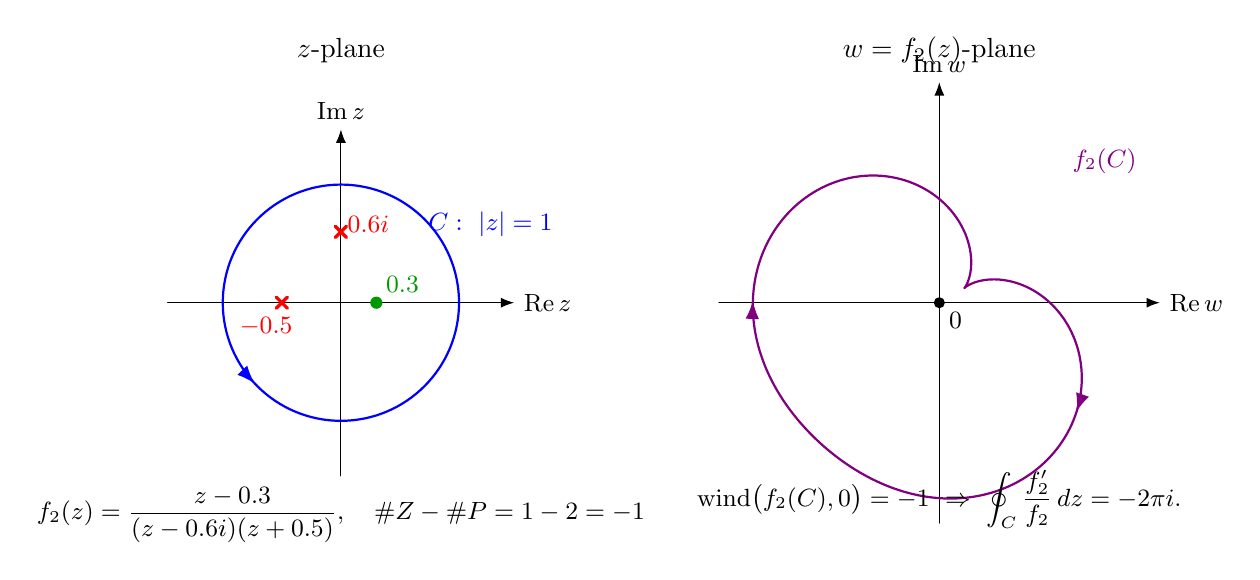
\begin{tikzpicture}[>=Latex, line cap=round, line join=round, font=\small]

% ==== Left: z-plane ====
\begin{scope}
	\node[font=\normalsize] at (0,3.2) {$z$-plane};
	\draw[->] (-2.2,0)--(2.2,0) node[right] {$\Re z$};
	\draw[->] (0,-2.2)--(0,2.2) node[above] {$\Im z$};
	
	% unit circle C
	\draw[blue,thick,postaction={decorate},
	decoration={markings, mark=at position 0.62 with {\arrow{>}}}]
	(0,0) circle (1.5);
	\node[blue] at (1.9,1.0) {$C:\ |z|=1$};
	
	% one zero inside
	\fill[green!60!black] (0.45,0) circle(2.2pt) node[above right] {$0.3$};
	
	% two poles inside: 0.6i and -0.5
	\draw[red,very thick] (0,0.9) ++(-0.07,-0.07) -- ++(0.14,0.14);
	\draw[red,very thick] (0,0.9) ++(-0.07,0.07) -- ++(0.14,-0.14);
	\node[red] at (0.35,1.0) {$0.6i$};
	
	\draw[red,very thick] (-0.75,0) ++(-0.07,-0.07) -- ++(0.14,0.14);
	\draw[red,very thick] (-0.75,0) ++(-0.07,0.07) -- ++(0.14,-0.14);
	\node[red] at (-0.95,-0.3) {$-0.5$};
	
	\node[align=left] at (0,-2.7) {$\displaystyle
		f_2(z)=\frac{z-0.3}{(z-0.6i)(z+0.5)},\quad \#Z-\#P=1-2=-1$};
\end{scope}

% ==== Right: w-plane ====
\begin{scope}[shift={(7.6,0)}]
	\node[font=\normalsize] at (0,3.2) {$w=f_2(z)$-plane};
	\draw[->] (-2.8,0)--(2.8,0) node[right] {$\Re w$};
	\draw[->] (0,-2.8)--(0,2.8) node[above] {$\Im w$};
	\fill (0,0) circle(2pt) node[below right] {$0$};
	
	% Param: z = e^{it} = x+iy, x=cos t, y=sin t
	% N = (x-0.3) + i y
	% D = (z-0.6i)(z+0.5) with
	%   D_re = x^2 + 0.5x - y^2 + 0.6y
	%   D_im = 2xy - 0.6x + 0.5y - 0.3
	% |D|^2 = D_re^2 + D_im^2
	\draw[violet,thick,
	postaction={decorate},
	decoration={markings, mark=at position 0.20 with {\arrow{>}},
		mark=at position 0.65 with {\arrow{>}}}]
	plot[domain=0:6.283, samples=650]
	({
		( (cos(\x r)-0.3) * ( (cos(\x r)*cos(\x r) + 0.5*cos(\x r) - sin(\x r)*sin(\x r) + 0.6*sin(\x r)) )
		+ ( sin(\x r) ) * ( 2*cos(\x r)*sin(\x r) - 0.6*cos(\x r) + 0.5*sin(\x r) - 0.3 )
		)
		/
		(
		(cos(\x r)*cos(\x r) + 0.5*cos(\x r) - sin(\x r)*sin(\x r) + 0.6*sin(\x r))^2
		+ (2*cos(\x r)*sin(\x r) - 0.6*cos(\x r) + 0.5*sin(\x r) - 0.3)^2
		)
	},
	{
		( sin(\x r) * ( (cos(\x r)*cos(\x r) + 0.5*cos(\x r) - sin(\x r)*sin(\x r) + 0.6*sin(\x r)) )
		- (cos(\x r)-0.3) * ( 2*cos(\x r)*sin(\x r) - 0.6*cos(\x r) + 0.5*sin(\x r) - 0.3 )
		)
		/
		(
		(cos(\x r)*cos(\x r) + 0.5*cos(\x r) - sin(\x r)*sin(\x r) + 0.6*sin(\x r))^2
		+ (2*cos(\x r)*sin(\x r) - 0.6*cos(\x r) + 0.5*sin(\x r) - 0.3)^2
		)
	});
	\node[violet] at (2.1,1.8) {$f_2(C)$};
	
	\node[align=center] at (0,-2.5)
	{$\mathrm{wind}\big(f_2(C),0\big)=-1
		\ \Rightarrow\ 
		\displaystyle \oint_C \frac{f_2'}{f_2}\,dz=-2\pi i.$};
\end{scope}

\end{tikzpicture}
\end{document}
